\tikzset{
  resistor/.style={thick,decorate,decoration={zigzag,segment length=4.2pt,amplitude=1.8pt}},
  circuitwire/.style={thick,Ink},
  samenode/.style={circle,draw=DeepBlue,fill=PaleBlue,inner sep=1.6pt},
  terminal/.style={circle,fill=DeepBlue,inner sep=2.2pt}
}

\newcommand{\sourceEquivalentDiagram}{%
\begin{center}
\begin{tikzpicture}[scale=0.88,>=Latex]
  \begin{scope}[xshift=-3.4cm]
    \draw[circuitwire] (-1.5,1)--(-0.45,1);
    \draw[very thick,DeepBlue] (-0.45,1.35)--(-0.45,0.65) (-0.08,1.24)--(-0.08,0.76);
    \draw[resistor] (-0.08,1)--(1.25,1);
    \draw[circuitwire] (1.25,1)--(1.55,1) (-1.5,-1)--(1.55,-1);
    \node at (-0.25,1.65) {$\mathcal E$}; \node at (0.65,1.45) {$r$};
    \node[terminal] at (-1.5,1){}; \node[terminal] at (-1.5,-1){};
  \end{scope}
  \draw[<->,DeepBlue,very thick] (-1.0,0)--(1.0,0)
    node[midway,above] {$\mathcal E=I_{\rm N}r$};
  \begin{scope}[xshift=3.4cm]
    \draw[circuitwire] (-1.5,1)--(1.45,1) (-1.5,-1)--(1.45,-1);
    \draw[circuitwire] (0.15,1)--(0.15,0.45) (0.15,-0.45)--(0.15,-1);
    \draw[resistor] (0.15,0.45)--(0.15,-0.45);
    \draw[circuitwire] (1.05,1)--(1.05,0.48) (1.05,-0.48)--(1.05,-1);
    \draw[DeepBlue,very thick,->] (1.05,-0.48)--(1.05,0.48);
    \node[left] at (-0.05,0) {$r$}; \node[right] at (1.25,0) {$I_{\rm N}$};
    \node[terminal] at (-1.5,1){}; \node[terminal] at (-1.5,-1){};
  \end{scope}
\end{tikzpicture}

{\small\color{TextGray}图 34.1\quad 实际电压源与实际电流源的端口等效}
\end{center}}

\newcommand{\theveninDiagram}{%
\begin{center}
\begin{tikzpicture}[scale=0.88,>=Latex]
  \draw[rounded corners=2mm,fill=PaleBlue,draw=RuleGray] (-4,-1.35) rectangle (-1.25,1.35);
  \node[align=center] at (-2.62,0) {任意线性\\有源二端网络};
  \draw[circuitwire] (-1.25,0.75)--(-0.65,0.75) (-1.25,-0.75)--(-0.65,-0.75);
  \node[terminal] at (-0.65,0.75){}; \node[terminal] at (-0.65,-0.75){};
  \draw[->,DeepBlue,very thick] (0,0)--(1.1,0);
  \draw[circuitwire] (1.6,0.75)--(2.1,0.75);
  \draw[very thick,DeepBlue] (2.1,1.1)--(2.1,0.4) (2.45,0.98)--(2.45,0.52);
  \draw[resistor] (2.45,0.75)--(3.75,0.75);
  \draw[circuitwire] (3.75,0.75)--(4.1,0.75) (1.6,-0.75)--(4.1,-0.75);
  \node at (2.3,1.35) {$U_{\rm oc}$}; \node at (3.15,1.2) {$R_{\rm th}$};
  \node[terminal] at (4.1,0.75){}; \node[terminal] at (4.1,-0.75){};
\end{tikzpicture}

{\small\color{TextGray}图 34.2\quad Thevenin 等效只保留开路电压与端口内阻}
\end{center}}

\newcommand{\bridgeDiagram}{%
\begin{center}
\begin{tikzpicture}[scale=0.9,>=Latex]
  \coordinate (L) at (-3,0); \coordinate (T) at (0,1.65);
  \coordinate (B) at (0,-1.65); \coordinate (R) at (3,0);
  \draw[resistor] (L)--node[above left] {$R_1$}(T);
  \draw[resistor] (T)--node[above right] {$R_2$}(R);
  \draw[resistor] (L)--node[below left] {$R_3$}(B);
  \draw[resistor] (B)--node[below right] {$R_4$}(R);
  \draw[resistor,DeepBlue] (T)--node[right] {$R_5$}(B);
  \fill[DeepBlue] (L) circle (2.5pt) node[left] {$A$};
  \fill[DeepBlue] (R) circle (2.5pt) node[right] {$B$};
  \node[TextGray,align=left,anchor=west] at (4.0,0.35)
    {$R_1/R_2=R_3/R_4$\\$\Rightarrow\ U_T=U_B$\\$\Rightarrow\ I_5=0$};
\end{tikzpicture}

{\small\color{TextGray}图 34.3\quad 平衡电桥的中间支路可断开，也可将两端等势点合并}
\end{center}}

\newcommand{\starDeltaDiagram}{%
\begin{center}
\begin{tikzpicture}[scale=0.86,>=Latex]
  \begin{scope}[xshift=-3.1cm]
    \coordinate (A) at (0,1.65); \coordinate (B) at (-1.7,-1.1); \coordinate (C) at (1.7,-1.1);
    \draw[resistor] (A)--node[left] {$R_{AB}$}(B);
    \draw[resistor] (B)--node[below] {$R_{BC}$}(C);
    \draw[resistor] (C)--node[right] {$R_{CA}$}(A);
    \node[above] at (A) {$A$}; \node[left] at (B) {$B$}; \node[right] at (C) {$C$};
  \end{scope}
  \draw[<->,DeepBlue,very thick] (-0.55,0)--(0.55,0);
  \begin{scope}[xshift=3.1cm]
    \coordinate (A) at (0,1.65); \coordinate (B) at (-1.7,-1.1); \coordinate (C) at (1.7,-1.1); \coordinate (O) at (0,0);
    \draw[resistor] (A)--node[right] {$R_A$}(O);
    \draw[resistor] (B)--node[above left] {$R_B$}(O);
    \draw[resistor] (C)--node[above right] {$R_C$}(O);
    \node[above] at (A) {$A$}; \node[left] at (B) {$B$}; \node[right] at (C) {$C$};
    \fill[DeepBlue] (O) circle (2.2pt);
  \end{scope}
\end{tikzpicture}

{\small\color{TextGray}图 34.4\quad 三角形连接与星形连接的端口等效}
\end{center}}

\newcommand{\gridDiagram}{%
\begin{center}
\begin{tikzpicture}[scale=0.8]
  \foreach \x in {0,1,2}{\draw[curve] (\x,0)--(\x,2);}
  \foreach \y in {0,1,2}{\draw[curve] (0,\y)--(2,\y);}
  \foreach \x in {0,1,2}{\foreach \y in {0,1,2}{\fill[Ink] (\x,\y) circle (1.5pt);}}
  \node[left] at (0,0) {$A$}; \node[right] at (2,0) {$B$}; \node[right] at (2,2) {$C$};
  \draw[->,DeepBlue] (3.0,1)--(4.25,1);
  \node[TextGray,align=left,anchor=west] at (4.6,1)
    {先按端点对称性分组\\再合并等势节点};
\end{tikzpicture}

{\small\color{TextGray}图 34.5\quad 田字格网络的节点与端点标记}
\end{center}}

\newcommand{\tetrahedronDiagram}{%
\begin{center}
\begin{tikzpicture}[scale=0.88]
  \coordinate (A) at (0,2); \coordinate (B) at (-2,-1.25);
  \coordinate (C) at (2,-1.25); \coordinate (D) at (0,-0.35);
  \foreach \u/\v in {A/B,A/C,A/D,B/C,B/D,C/D}{\draw[curve] (\u)--(\v);}
  \foreach \u/\pos in {A/above,B/left,C/right,D/below}{\fill[DeepBlue] (\u) circle (2.3pt) node[\pos] {$\u$};}
  \node[TextGray,anchor=west,align=left] at (3.0,0.35)
    {从 $A$ 流入、从 $B$ 流出时\\$C,D$ 关于交换对称，故等势};
\end{tikzpicture}

{\small\color{TextGray}图 34.6\quad 正四面体六条棱均接电阻 $R$}
\end{center}}

\newcommand{\completeGraphDiagram}{%
\begin{center}
\begin{tikzpicture}[scale=0.82]
  \foreach \i in {0,...,4}{\coordinate (P\i) at ({90+72*\i}:1.8);}
  \foreach \i in {0,...,4}{\foreach \j in {0,...,4}{\ifnum\i<\j\draw[curve] (P\i)--(P\j);\fi}}
  \foreach \i in {0,...,4}{\fill[DeepBlue] (P\i) circle (2.2pt);}
  \node[TextGray,anchor=west,align=left] at (3.0,0.35)
    {$K_N$ 中任意两点都有一只 $R$\\其余 $N-2$ 个节点彼此等势};
\end{tikzpicture}

{\small\color{TextGray}图 34.7\quad $N=5$ 时的完全图电阻网络}
\end{center}}

\newcommand{\octagonDiagram}{%
\begin{center}
\begin{tikzpicture}[scale=0.75]
  \foreach \i in {0,...,7}{\coordinate (O\i) at ({22.5+45*\i}:2.25);}
  \foreach \i in {0,...,7}{\foreach \j in {0,...,7}{
    \pgfmathtruncatemacro{\d}{mod(\j-\i+8,8)}
    \ifnum\i<\j\ifnum\d=4\else\draw[thin,TextGray] (O\i)--(O\j);\fi\fi}}
  \foreach \i in {0,...,7}{\fill[Ink] (O\i) circle (1.7pt);}
  \fill[DeepBlue] (O0) circle (3pt) node[right] {$A$};
  \fill[DeepBlue] (O4) circle (3pt) node[left] {$B$};
  \node[TextGray,anchor=west,align=left] at (3.7,0.3)
    {删去四条最长对角线\\求对径端点 $A,B$ 间电阻};
\end{tikzpicture}

{\small\color{TextGray}图 34.8\quad 变种八边形：除对径点外任意两点均以 $R$ 相连}
\end{center}}

\newcommand{\cubeDiagram}{%
\begin{center}
\begin{tikzpicture}[scale=0.82]
  \coordinate (A) at (-2,-1.3); \coordinate (B) at (1,-1.3);
  \coordinate (C) at (1,1.5); \coordinate (D) at (-2,1.5);
  \coordinate (E) at (-0.8,-0.35); \coordinate (F) at (2.2,-0.35);
  \coordinate (G) at (2.2,2.45); \coordinate (H) at (-0.8,2.45);
  \foreach \u/\v in {A/B,B/C,C/D,D/A,E/F,F/G,G/H,H/E,A/E,B/F,C/G,D/H}{\draw[curve] (\u)--(\v);}
  \draw[guide] (E)--(F) (E)--(H) (A)--(E);
  \foreach \u in {A,B,C,D,E,F,G,H}{\fill[Ink] (\u) circle (1.7pt);}
  \node[left] at (A) {$A$}; \node[below] at (B) {$B$}; \node[right] at (C) {$C$}; \node[above] at (G) {$C_1$};
  \node[TextGray,anchor=west,align=left] at (3.25,0.55)
    {棱相邻：$A,B$\\面对角：$A,C$\\体对角：$A,G$};
\end{tikzpicture}

{\small\color{TextGray}图 34.9\quad 正方体十二条棱均接电阻 $R$}
\end{center}}

\newcommand{\ladderDiagram}{%
\begin{center}
\begin{tikzpicture}[scale=0.78]
  \node[left] at (0,1.2) {$a$}; \node[left] at (0,-1.2) {$b$};
  \foreach \i in {0,1,2,3}{
    \draw[resistor] (1.45*\i,1.2)--(1.45*\i+1.05,1.2);
    \draw[resistor] (1.45*\i,-1.2)--(1.45*\i+1.05,-1.2);
    \draw[resistor] (1.45*\i+1.05,1.2)--(1.45*\i+1.05,-1.2);
    \fill[Ink] (1.45*\i+1.05,1.2) circle (1.4pt);
    \fill[Ink] (1.45*\i+1.05,-1.2) circle (1.4pt);
  }
  \draw[dotted,thick] (5.7,1.2)--(6.45,1.2) (5.7,-1.2)--(6.45,-1.2);
\end{tikzpicture}

{\small\color{TextGray}图 34.10\quad 每一节含上下两个串联电阻和一只横接电阻}
\end{center}}

\newcommand{\threeRailDiagram}{%
\begin{center}
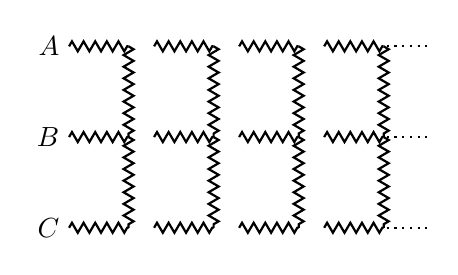
\begin{tikzpicture}[scale=0.72]
  \foreach \row/\lab in {1.6/A,0/B,-1.6/C}{\node[left] at (0,\row) {$\lab$};}
  \foreach \i in {0,1,2,3}{
    \foreach \row in {1.6,0,-1.6}{\draw[resistor] (1.5*\i,\row)--(1.5*\i+1.05,\row);}
    \draw[resistor] (1.5*\i+1.05,1.6)--(1.5*\i+1.05,0);
    \draw[resistor] (1.5*\i+1.05,0)--(1.5*\i+1.05,-1.6);
  }
  \foreach \row in {1.6,0,-1.6}{\draw[dotted,thick] (5.6,\row)--(6.35,\row);}
\end{tikzpicture}

{\small\color{TextGray}图 34.11\quad 三端无限方格网络及端点 $A,B,C$}
\end{center}}

\newcommand{\nestedTriangleDiagram}{%
\begin{center}
\begin{tikzpicture}[scale=0.85]
  \coordinate (A) at (-3,-1.55); \coordinate (B) at (3,-1.55); \coordinate (C) at (0,3.65);
  \draw[curve] (A)--(B)--(C)--cycle;
  \coordinate (L1) at (-1.5,1.05); \coordinate (R1) at (1.5,1.05); \coordinate (M1) at (0,-1.55);
  \draw[curve] (L1)--(R1)--(M1)--cycle;
  \coordinate (L2) at (-0.75,-0.25); \coordinate (R2) at (0.75,-0.25); \coordinate (M2) at (0,1.05);
  \draw[curve] (L2)--(R2)--(M2)--cycle;
  \coordinate (L3) at (-0.375,0.40); \coordinate (R3) at (0.375,0.40); \coordinate (M3) at (0,-0.25);
  \draw[curve] (L3)--(R3)--(M3)--cycle;
  \node[left] at (A) {$A$}; \node[right] at (B) {$B$}; \node[above] at (C) {$C$};
  \node[TextGray,anchor=west,align=left] at (4.0,0.65)
    {边长依次为\\$a,a/2,a/4,\ldots$};
\end{tikzpicture}

{\small\color{TextGray}图 34.12\quad 相邻内接等边三角形在三个中点处与外层相接}
\end{center}}

\newcommand{\sierpinskiDiagram}{%
\begin{center}
\begin{tikzpicture}[scale=0.78]
  \begin{scope}[xshift=-3.4cm]
    \fill[PaleBlue] (-1.7,-1.1)--(1.7,-1.1)--(0,1.84)--cycle;
    \node[below] at (0,-1.45) {第 0 阶};
  \end{scope}
  \begin{scope}
    \fill[PaleBlue] (-1.7,-1.1)--(0,-1.1)--(-0.85,0.37)--cycle;
    \fill[PaleBlue] (0,-1.1)--(1.7,-1.1)--(0.85,0.37)--cycle;
    \fill[PaleBlue] (-0.85,0.37)--(0.85,0.37)--(0,1.84)--cycle;
    \draw[curve] (-1.7,-1.1)--(1.7,-1.1)--(0,1.84)--cycle;
    \node[below] at (0,-1.45) {第 1 阶};
  \end{scope}
  \begin{scope}[xshift=3.4cm]
    \foreach \sx/\sy in {-1.275/-0.735,0/-0.735,-0.6375/0.3675}{
      \fill[PaleBlue] (\sx-0.425,\sy-0.3675)--(\sx+0.425,\sy-0.3675)--(\sx,\sy+0.3675)--cycle;
    }
    \foreach \sx/\sy in {-0.425/-0.735,0.85/-0.735,0.425/0.3675}{
      \fill[PaleBlue] (\sx-0.425,\sy-0.3675)--(\sx+0.425,\sy-0.3675)--(\sx,\sy+0.3675)--cycle;
    }
    \fill[PaleBlue] (-0.425,0.735)--(0.425,0.735)--(0,1.47)--cycle;
    \draw[curve] (-1.7,-1.1)--(1.7,-1.1)--(0,1.84)--cycle;
    \node[below] at (0,-1.45) {第 2 阶};
  \end{scope}
\end{tikzpicture}

{\small\color{TextGray}图 34.13\quad 谢尔宾斯基镂垫的前几阶构造}
\end{center}}
